\documentclass[a4paper]{report}
% Some basic packages
\usepackage[utf8]{inputenc}
\usepackage[T1]{fontenc}
\usepackage{textcomp}
\usepackage[english]{babel}
\usepackage{url}
\usepackage{graphicx}
\usepackage{float}
\usepackage{booktabs}
\usepackage{enumitem}

\pdfminorversion=7

% Don't indent paragraphs, leave some space between them
\usepackage{parskip}

% Hide page number when page is empty
\usepackage{emptypage}
\usepackage{subcaption}
\usepackage{multicol}
\usepackage{xcolor}

% Other font I sometimes use.
% \usepackage{cmbright}

% Math stuff
\usepackage{amsmath, amsfonts, mathtools, amsthm, amssymb}
% Fancy script capitals
\usepackage{mathrsfs}
\usepackage{cancel}
% Bold math
\usepackage{bm}
% Some shortcuts
\newcommand\N{\ensuremath{\mathbb{N}}}
\newcommand\R{\ensuremath{\mathbb{R}}}
\newcommand\Z{\ensuremath{\mathbb{Z}}}
\renewcommand\O{\ensuremath{\emptyset}}
\newcommand\Q{\ensuremath{\mathbb{Q}}}
\newcommand\C{\ensuremath{\mathbb{C}}}
\renewcommand\L{\ensuremath{\mathcal{L}}}

% Package for Petri Net drawing
\usepackage[version=0.96]{pgf}
\usepackage{tikz}
\usetikzlibrary{arrows,shapes,automata,petri}
\usepackage{tikzit}
\input{petri_nets_style.tikzstyles}

% Easily typeset systems of equations (French package)
\usepackage{systeme}

% Put x \to \infty below \lim
\let\svlim\lim\def\lim{\svlim\limits}

%Make implies and impliedby shorter
\let\implies\Rightarrow
\let\impliedby\Leftarrow
\let\iff\Leftrightarrow
\let\epsilon\varepsilon

% Add \contra symbol to denote contradiction
\usepackage{stmaryrd} % for \lightning
\newcommand\contra{\scalebox{1.5}{$\lightning$}}

% \let\phi\varphi

% Command for short corrections
% Usage: 1+1=\correct{3}{2}

\definecolor{correct}{HTML}{009900}
\newcommand\correct[2]{\ensuremath{\:}{\color{red}{#1}}\ensuremath{\to }{\color{correct}{#2}}\ensuremath{\:}}
\newcommand\green[1]{{\color{correct}{#1}}}

% horizontal rule
\newcommand\hr{
    \noindent\rule[0.5ex]{\linewidth}{0.5pt}
}

% hide parts
\newcommand\hide[1]{}

% si unitx
\usepackage{siunitx}
\sisetup{locale = FR}

% Environments
\makeatother
% For box around Definition, Theorem, \ldots
\usepackage{mdframed}
\mdfsetup{skipabove=1em,skipbelow=0em}
\theoremstyle{definition}
\newmdtheoremenv[nobreak=true]{definitie}{Definitie}
\newmdtheoremenv[nobreak=true]{eigenschap}{Eigenschap}
\newmdtheoremenv[nobreak=true]{gevolg}{Gevolg}
\newmdtheoremenv[nobreak=true]{lemma}{Lemma}
\newmdtheoremenv[nobreak=true]{propositie}{Propositie}
\newmdtheoremenv[nobreak=true]{stelling}{Stelling}
\newmdtheoremenv[nobreak=true]{wet}{Wet}
\newmdtheoremenv[nobreak=true]{postulaat}{Postulaat}
\newmdtheoremenv{conclusie}{Conclusie}
\newmdtheoremenv{toemaatje}{Toemaatje}
\newmdtheoremenv{vermoeden}{Vermoeden}
\newtheorem*{herhaling}{Herhaling}
\newtheorem*{intermezzo}{Intermezzo}
\newtheorem*{notatie}{Notatie}
\newtheorem*{observatie}{Observatie}
\newtheorem*{exe}{Exercise}
\newtheorem*{opmerking}{Opmerking}
\newtheorem*{praktisch}{Praktisch}
\newtheorem*{probleem}{Probleem}
\newtheorem*{terminologie}{Terminologie}
\newtheorem*{toepassing}{Toepassing}
\newtheorem*{uovt}{UOVT}
\newtheorem*{vb}{Voorbeeld}
\newtheorem*{vraag}{Vraag}

\newmdtheoremenv[nobreak=true]{definition}{Definition}
\newtheorem*{eg}{Example}
\newtheorem*{notation}{Notation}
\newtheorem*{previouslyseen}{As previously seen}
\newtheorem*{remark}{Remark}
\newtheorem*{note}{Note}
\newtheorem*{problem}{Problem}
\newtheorem*{observe}{Observe}
\newtheorem*{property}{Property}
\newtheorem*{intuition}{Intuition}
\newmdtheoremenv[nobreak=true]{prop}{Proposition}
\newmdtheoremenv[nobreak=true]{theorem}{Theorem}
\newmdtheoremenv[nobreak=true]{corollary}{Corollary}

% End example and intermezzo environments with a small diamond (just like proof
% environments end with a small square)
\usepackage{etoolbox}
\AtEndEnvironment{vb}{\null\hfill$\diamond$}%
\AtEndEnvironment{intermezzo}{\null\hfill$\diamond$}%
% \AtEndEnvironment{opmerking}{\null\hfill$\diamond$}%

% Fix some spacing
% http://tex.stackexchange.com/questions/22119/how-can-i-change-the-spacing-before-theorems-with-amsthm
\makeatletter
\def\thm@space@setup{%
  \thm@preskip=\parskip \thm@postskip=0pt
}


% Exercise 
% Usage:
% \exercise{5}
% \subexercise{1}
% \subexercise{2}
% \subexercise{3}
% gives
% Exercise 5
%   Exercise 5.1
%   Exercise 5.2
%   Exercise 5.3
\newcommand{\exercise}[1]{%
    \def\@exercise{#1}%
    \subsection*{Exercise #1}
}

\newcommand{\subexercise}[1]{%
    \subsubsection*{Exercise \@exercise.#1}
}


% \lecture starts a new lecture (les in dutch)
%
% Usage:
% \lecture{1}{di 12 feb 2019 16:00}{Inleiding}
%
% This adds a section heading with the number / title of the lecture and a
% margin paragraph with the date.

% I use \dateparts here to hide the year (2019). This way, I can easily parse
% the date of each lecture unambiguously while still having a human-friendly
% short format printed to the pdf.

\usepackage{xifthen}
\def\testdateparts#1{\dateparts#1\relax}
\def\dateparts#1 #2 #3 #4 #5\relax{
    \marginpar{\small\textsf{\mbox{#1 #2 #3 #5}}}
}

\def\@lecture{}%
\newcommand{\lecture}[3]{
    \ifthenelse{\isempty{#3}}{%
        \def\@lecture{Lecture #1}%
    }{%
        \def\@lecture{Lecture #1: #3}%
    }%
    \subsection*{\@lecture}
    \marginpar{\small\textsf{\mbox{#2}}}
}



% These are the fancy headers
\usepackage{fancyhdr}
\pagestyle{fancy}

% LE: left even
% RO: right odd
% CE, CO: center even, center odd
% My name for when I print my lecture notes to use for an open book exam.
% \fancyhead[LE,RO]{Gilles Castel}

\fancyhead[RO,LE]{\@lecture} % Right odd,  Left even
\fancyhead[RE,LO]{}          % Right even, Left odd

\fancyfoot[RO,LE]{\thepage}  % Right odd,  Left even
\fancyfoot[RE,LO]{}          % Right even, Left odd
\fancyfoot[C]{\leftmark}     % Center

\makeatother




% Todonotes and inline notes in fancy boxes
\usepackage{todonotes}
\usepackage{tcolorbox}

% Make boxes breakable
\tcbuselibrary{breakable}

% Verbetering is correction in Dutch
% Usage: 
% \begin{verbetering}
%     Lorem ipsum dolor sit amet, consetetur sadipscing elitr, sed diam nonumy eirmod
%     tempor invidunt ut labore et dolore magna aliquyam erat, sed diam voluptua. At
%     vero eos et accusam et justo duo dolores et ea rebum. Stet clita kasd gubergren,
%     no sea takimata sanctus est Lorem ipsum dolor sit amet.
% \end{verbetering}
\newenvironment{verbetering}{\begin{tcolorbox}[
    arc=0mm,
    colback=white,
    colframe=green!60!black,
    title=Opmerking,
    fonttitle=\sffamily,
    breakable
]}{\end{tcolorbox}}

% Noot is note in Dutch. Same as 'verbetering' but color of box is different
\newenvironment{noot}[1]{\begin{tcolorbox}[
    arc=0mm,
    colback=white,
    colframe=white!60!black,
    title=#1,
    fonttitle=\sffamily,
    breakable
]}{\end{tcolorbox}}




% Figure support as explained in my blog post.
\usepackage{import}
\usepackage{xifthen}
\usepackage{pdfpages}
\usepackage{transparent}
\newcommand{\incfig}[1]{%
    \def\svgwidth{\columnwidth}
    \import{./figures/}{#1.pdf_tex}
}

% Fix some stuff
% %http://tex.stackexchange.com/questions/76273/multiple-pdfs-with-page-group-included-in-a-single-page-warning
\pdfsuppresswarningpagegroup=1


% My name
\author{Bruno M. Pacheco}

 
\begin{document}
 
\title{Lista 2}
\author{Bruno M. Pacheco (16100865)\\
DAS5151 - Instrumentação em Controle}
 
\maketitle
 
\exercise{1}

Um termorresistor, por natureza, é bastante impactado pela resistência dos condutores quando medido a 2 fios, e.g., quando utiliza-se uma fonte de corrente e um voltímetro, a queda de tensão nos condutores é somada a queda de tensão no termorresistor o que causa um \emph{offset} no valor medido.

Para evitar tal erro, uma medição a 4 fios, por exemplo, aplica-se a corrente através de um par de condutores enquanto mede-se a tensão através de outro par, evitando a queda de tensão nos condutores que conectam o termorresistor ao voltímetro, ou seja, mede-se somente a queda de tensão sobre o termorresistor.

Uma outra possibilidade é utilizar uma segunda fonte de corrente e realizar uma medição a 3 fios. Nessa configuração, as duas fontes de corrente são utilizadas para gerar uma quedas de tensão no sentido contrário (em relação à malha do voltímetro) nos condutores que encontram-se entre o termorresistor e o voltímetro. Dessa forma, se as resistências dos condutores são idênticas e garante-se que as fontes de corrente injetam a mesma corrente no circuito, o erro é compensado no próprio circuito (a queda de tensão em um condutor é de mesma intensidade mas oposta à queda de tensão no outro).

\exercise{2}

\subexercise{a}

A partir da temperatura $T_r$ encontra-se a tensão $V_r = 0,912\,mV$. Dessa forma, pode-se encontrar a tensão gerada pela junção na temperatura $T_j$, ou seja, $V_j = 1,796+0,912 = 2,708\,mV$. Assim, encontra-se uma temperatura $T_j = 65,44\,^\circ C$.

\subexercise{b}

Um valor fixo do coeficiente de Seebeck poderia ser uma boa aproximação, mas como sabemos que esse coeficiente varia de acordo com a temperatura, teríamos um erro maior do que a curva fornecida pela tabela, afinal, utilizar um coeficiente de Seebeck fixo é o mesmo que aproximar a variação de temperatura por um polinômio de grau 1.

No caso da aplicação proposta, por exemplo, utilizando o coeficiente fornecido, ter-se-ia um erro de cerca de 2 \% na temperatura estimada para valores de tensão próximos do enunciado.

\exercise{3}

A partir do CMRR fornecido e do ganho de malha direta, tem-se \[
    100 = 20 \log \left|\frac{100}{A_{cm}}\right| \implies A_{cm} = 10^{-3}
.\] Dessa forma, pode-se estimar \[
V_o = A_d\left( V^{+}-V^{-} \right) + A_{cm}\left( \frac{V^{+}+V^{-}}{2} \right) = 1,01\,V
.\] 

\exercise{4}

Assumindo valores típicos de $10^5$ e $90\,dB$ para o ganho de malha aberta e o CMRR do LM741, podemos comparar com os valores encontrados no INA118 sem um resistor para controle do ganho. De acordo com informações do fabricante (datasheet da TI), o INA118 sem um resistor $R_G$ (pinos 1 e 8 desconectados) possui ganho unitário e CMRR típico de $90\,dB$. Ou seja, apesar de um CMRR parecido, a diferença no ganho de malha aberta é praticamente impeditiva no que tange o seu uso para a maioria das aplicações em que se utilizaria o LM741, de ganho $10^5$.

\exercise{5}

Os circuitos como vistos pelo multímetro podem ser vistos na figura abaixo.

\begin{figure}[H]
    \centering
    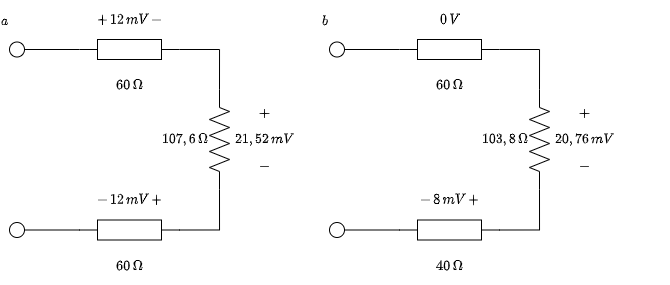
\includegraphics[width=0.8\textwidth]{lista2_5.png}
\end{figure}

\subexercise{a}

Para o primeiro cenário, o voltímetro mede $45,52\,mV$ o que seria convertido em $335,79\,^\circ C$.

\subexercise{b}

No segundo cenário, o voltímetro mede $28,76\,mV$, o que pode ser convertido para $115,26\,^\circ C$.

\exercise{6}

Denominando a impedância de entrada como $R_{in}$, sabemos que \[
V_{DAQ} = V_{FONTE} \frac{R_{in}}{R +R_{in}} \implies R_{in} = \frac{R V_{DAQ}}{V_{FONTE} - V_{DAQ}}
.\] 

Dessa forma, para $R=1\,k\Omega$ e $V_{FONTE} = 1,0\,V$, estima-se o impacto da variação de 0,99 para 0,98 no valor da tensão $V_{DAQ}$ para o cálculo da impedância de entrada de acordo com a equação anterior. Através desse método, chega-se em uma variação de $50\,k\Omega$. Da mesma forma mas para $V_{FONTE} = 5,0\,V$ e $V_{DAQ}$ de $4,94\,V$ para $4,93\,V$, estima-se um impacto de $\approx 11,9\,k\Omega$. Para $R=100\,k\Omega$ estima-se um impacto de $3,5\,k\Omega$ e $720\,\Omega$ para $V_{FONTE}$ em $1$ e $5\,V$, respectivamente.

A partir disso, utiliza-se os resultados de $R=100\,k\Omega$ e $V_{FONTE}=5\,V$, a partir dos quais determina-se $R_{in} \approx 90,1\,k\Omega$.

\exercise{7}

Como os termistores geralmente apresentam uma variação de resistência bastante alta dentro da faixa de medição especificada, uma medição a partir de um divisor resistivo é efetiva. Entretanto, o mesmo não acontece no caso de termorresistores do tipo PT100, por isso diferentes abordagens são necessárias para a aquisição.

\exercise{8}

\begin{enumerate}[label=\alph*]
    \item $4887,6\,\mu V$
    \item $305,2\,\mu V$
    \item $76,3\,\mu V$
    \item $0,3\,\mu V$
\end{enumerate}

\end{document}
